\section{Training time trade-offs in rapid development}

\begin{figure}[hbtp]
	\centering
	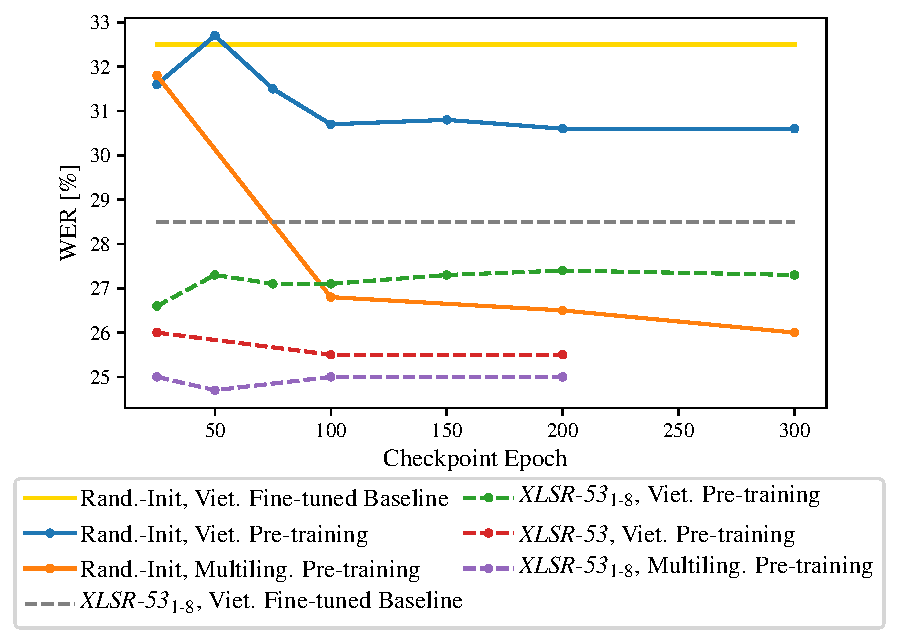
\includegraphics[width=1.0\textwidth]{figures/pretrain_comparison.pdf}
	\caption{
	    \glsxtrshort{WER} comparison using several pre-training checkpoints fine-tuned on the same schedule. 
	    The quantity of pre-training epochs is represented on the horizontal axis. 
	    The vertical axis displays the \glsxtrshort{WER} obtained after optimizing the Vietnamese in-house system on HYKIST dev data till convergence and evaluated on the initialization checkpoint that corresponds to it. 
	    All the pre-trainings in Vietnamese have been done using in-house data, not \glsxtrshort{YT} data. 
	    Keep in mind that if utilizing as an initialization, the training epochs for that model are not taken into consideration.
	    }
	\label{fig:fine_tune_comp_joint}
\end{figure}

It is vital to identify a trade-off between training time allowed and potential system performance while constructing \glsxtrshort{ASR} systems quickly. 
In this section, we examine the models that are most useful for this purpose. 
One epoch of pre-training on our internal Vietnamese data may be assumed to take around an hour on an NVIDIA 2080 GPU, but one epoch of fine-tuning can be estimated to take about three hours on the same setup. 
In our trials, the needed pre-training time scaled linearly with the amount of data.

Figure \ref{fig:fine_tune_comp_joint} compares various training methods using a hold-out dev dataset.
Yellow represents the baseline when fine-tuning from scratch.
Although pre-training using the in-house Vietnamese data (blue) results in a tiny improvement, it converges and stops improving after 100 iterations.
This is true even when the unsupervised loss is still improving.
Contrarily, the multilingual pre-training (orange) performs much better than the monolingual pre-training and enhances downstream \glsxtrshort{WER} even over prolonged training time.

Vietnamese \textit{XLSR-53}\textsubscript{1-8} (grey) fine-tuning is a very cost-effective training method that outperforms starting from scratch or pre-training on monolingual in-house data while utilizing only 26 training epochs in total.
Please take note that since the original \glsxtrshort{XLSR-53} model is available to the public, we do not count training epochs.
Although it requires more training time, using \glsxtrshort{XLSR-53} as an initialization for additional custom pre-training results in considerable \glsxtrshort{WERR} (green, red, purple).
It is evident from Figure \ref{fig:fine_tune_comp_joint} that even a brief pre-training with a few epochs produces significant benefits.
Consequently, this can be viewed as a quick and affordable solution to improve the performance of the model.
When employing data that is multilingual, the \glsxtrshort{WERR} is very potent.
Despite the fact that we have more data in this instance and a lengthier pre-training as a result, we only need to conduct this procedure once for all languages, making the situation essentially a zero-sum game.

In conclusion, it is clear that using the \glsxtrshort{XLSR-53} model to construct high-performing \glsxtrshort{ASR} models is very cost-effective. 
A quick multilingual pre-training that is helpful for downstream fine-tuning in all languages can further enhance performance.